\documentclass[tikz,border=10pt]{standalone}
\usepackage{tkz-euclide} % 用于简化几何点定位

\begin{document}
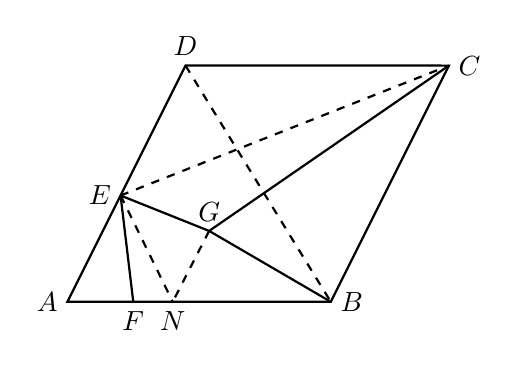
\begin{tikzpicture}[>=stealth, scale=1.5]
    % 1. 定义核心顶点坐标 (基于图像比例估算)
    \coordinate (A) at (0,0);
    \coordinate (B) at (2.23,0);
    \coordinate (D) at (1,2);
    \coordinate (C) at ($(B)+(D)-(A)$); % 平行四边形顶点C

    % 2. 定义边上的特殊点
    \coordinate (E) at ($(A)!0.45!(D)$);    % 点E在AD上
    \coordinate (F) at ($(A)!0.25!(B)$);    % 点F在AB上
    \coordinate (N) at ($(A)!0.4!(B)$);     % 点N在AB上
    \coordinate (G) at (1.2,0.6);            % 内部点G (估算位置)

    % 3. 绘制实线边框和主要连线
    \draw[thick] (A) -- (B) -- (C) -- (D) -- cycle; % 平行四边形外框
    \draw[thick] (E) -- (F);           % 连线 EF
    \draw[thick] (E) -- (G) -- (B);    % 连线 E-G-B
    \draw[thick] (G) -- (C);           % 连线 G-C

    % 4. 绘制虚线（辅助线或遮挡线）
    \draw[dashed, thick] (E) -- (N);   % 虚线 EN
    \draw[dashed, thick] (G) -- (N);   % 虚线 GN
    \draw[dashed, thick] (E) -- (C);   % 虚线 EC
    \draw[dashed, thick] (D) -- (B);   % 虚线 DB

    % 5. 标注字母标签
    \node[left] at (A) {$A$};
    \node[right] at (B) {$B$};
    \node[right] at (C) {$C$};
    \node[above] at (D) {$D$};
    \node[left] at (E) {$E$};
    \node[below] at (F) {$F$};
    \node[below] at (N) {$N$};
    \node[above] at (G) {$G$};

    % (可选) 标注点的位置，如需强调点可以取消下方注释
    %\foreach \p in {A,B,C,D,E,F,G,N} \fill (\p) circle (1pt);

\end{tikzpicture}
\end{document}